%! TEX root = ../main.tex
\documentclass[main]{subfiles}

\begin{document}
\section{Introduction}

An elliptic curve defined over a field $K$ of characteristic $\neq 2$ is a curve defined by a Weierstrass equation
\begin{equation*}
    E: y^{2} = x^{3} + Ax^2 + Bx + C
\end{equation*}
where $A,B,C \in K$ and the discriminant $\Delta = -4A^3C + A^2B^2 + 18ABC - 4B^3 - 27C^2$ is nonzero.
On points on an elliptic curve defined over $\mathbb{Q}$, we can define an addition law geometrically as follows.
\begin{figure}[H]
    \centering
    \caption{$E: y^2 = x(x-3^2)(x+4^2)$}
    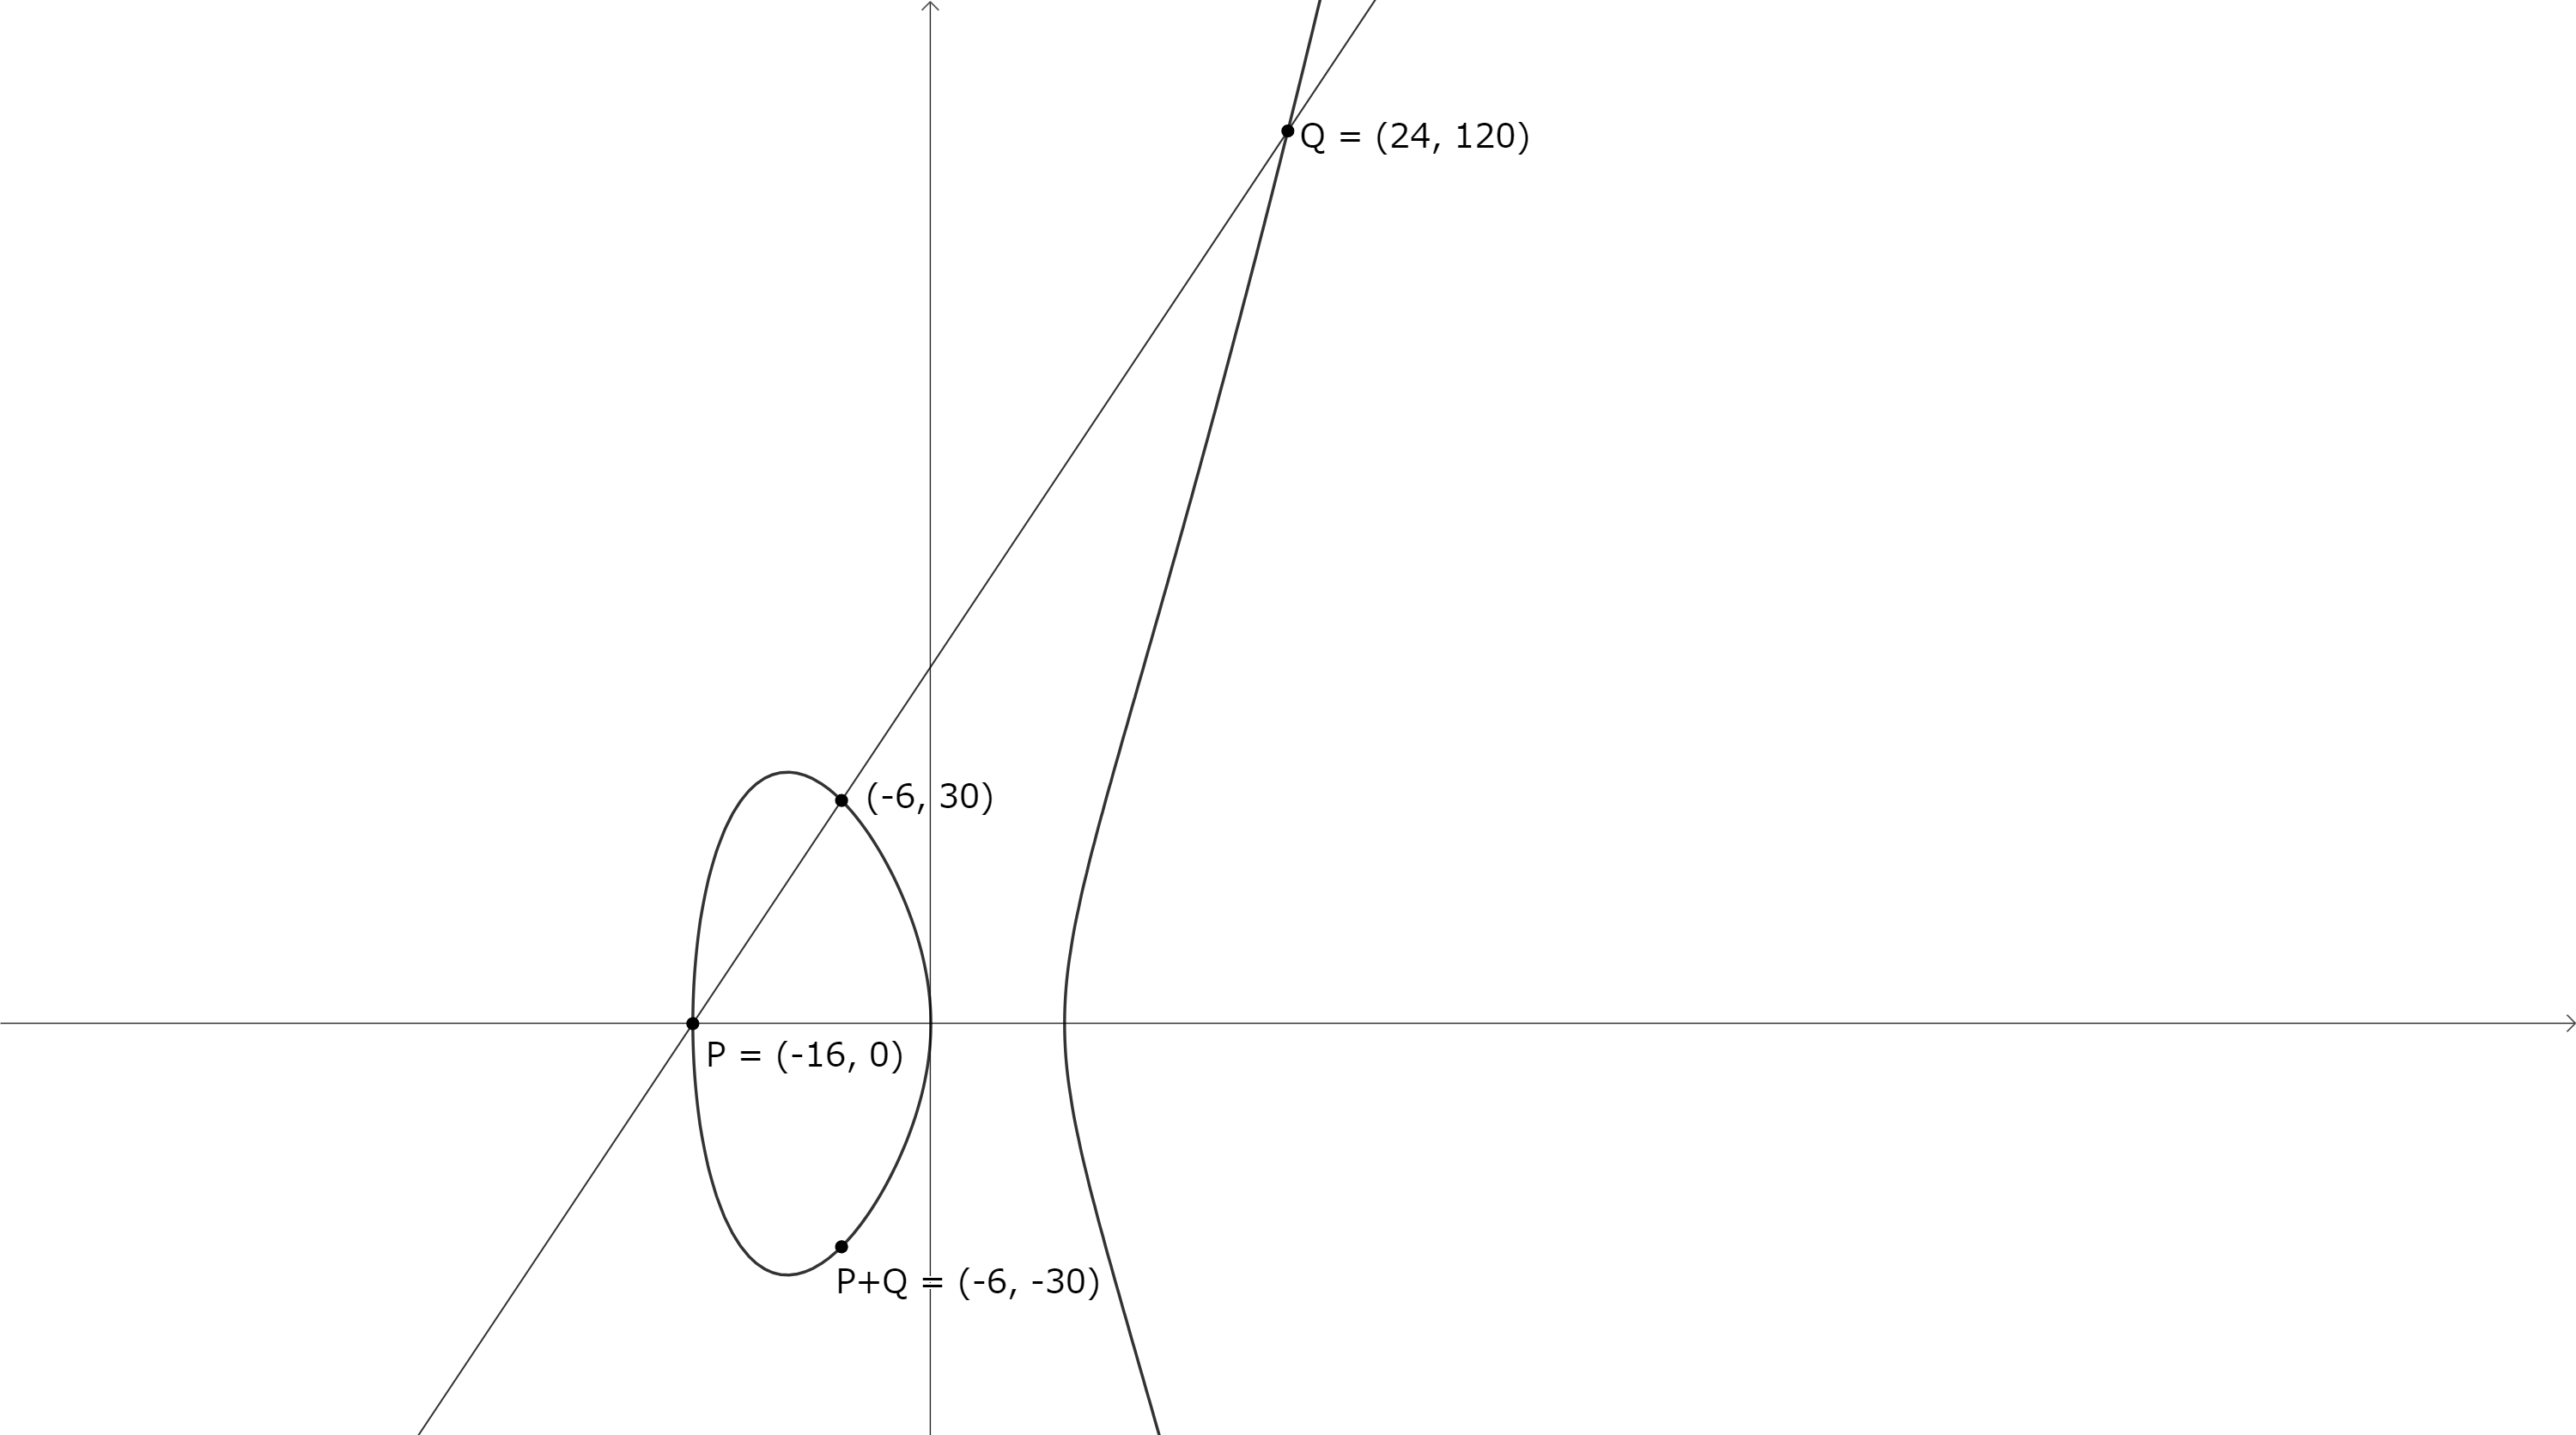
\includegraphics[keepaspectratio, width=\linewidth]{figures/3-4-5.png}
    \label{fig:elliptic_curve}
\end{figure}
For two points $P,Q$ on $E$, the point $-(P+Q)$ is defined as the third point of intersection of the line passing through $P$ and $Q$ with the curve.
The sum $P+Q$ is the point symmetric to $-(P+Q)$ with respect to the $x$-axis.
The definition can be extended to any field $K$ of characteristic $\neq 2$.
The set of points on an elliptic curve forms an abelian group with the identity element being the point at infinity.
The Mordell-Weil group $E(K)$ is a group consisting of all $K$-rational points on $E$.

\begin{prop}
    The kernel of multiplication by $2$ map $[2]: E(K) \to E(K)$ is
    \begin{equation*}
        E(K)[2] = \{ \mathcal{O} \} \cup \{ (x,y) \in E(K) \mid y = 0 \}.
    \end{equation*}
\end{prop}

\begin{thm}{(Mordell-Weil's Theorem)}
    \label{thm:mordell}
    Let $E$ be an elliptic curve defined over a number field $K$.
    Then the Mordell-Weil group $E(K)$ is a finitely generated abelian group.
\end{thm}
By the structure theorem of finite abelian groups, the Mordell-Weil group can be decomposed into a free part and a torsion part:
\begin{equation*}
    E(K) \cong \mathbb{Z}^{\oplus r} \oplus E(K)_{\text{tors}}
\end{equation*}
where $r$ is the rank of the Mordell-Weil group and $E(K)_{\text{tors}}$ is the torsion subgroup of $E(K)$.
The Mordell-Weil group is an important object in the arithmetic of elliptic curves.
Especially, the rank of the Mordell-Weil group is important and difficult to determine, in general.

Let $a,b,c$ be positive integers which satisfy the Fermat's equation
\begin{equation*}
    a^{n} + b^{n} = c^{n}.
\end{equation*}
for any integer $n \geq 2$ and consider the elliptic curve defined by the Weierstrass equation
\begin{equation*}
    y^{2} = x(x - a^{n})(x + b^{n}),
\end{equation*}
which is called the Frey curve.
The Frey curve played an important role in the proof of Fermat's Last Theorem by Wiles.
Wiles proved that the Frey curves do not exist for $n \geq 3$, which implies that the Fermat's equation has no nontrivial solution.

In this paper, we consider the case $n=2$ of the Frey curves.
In other words, let $(a,b,c) \in \mathbb{Z}_{> 0}^3$ be a Pythagorean triple and consider the elliptic curve defined by the Weierstrass equation
\begin{equation}
    \label{eq:2frey}
    y^{2} = x(x - a^{2})(x + b^{2}),
\end{equation}
which we call the Frey curve of degree $2$.
The Frey curves of degree $2$ do exist infinitely.

We can parameterize Pythagorean triples $(a,b,c)$ by $m,n \in \mathbb{Z}$ with $(m,n)=1$ as $(a,b,c) = (2mn, m^{2} - n^{2}, m^{2} + n^{2})$.
Then the equation \eqref{eq:2frey} can be written as $y^{2} = x(x - 4m^2n^2)(x + (m^{2} - n^2)^{2})$.
We replace $x,y$ by $n^2x, n^3y$ and put $s = m/n$.
Then we get an elliptic curve
\begin{equation}
    \label{eq:E_{1,s}}
    E_{1,s}: y^{2} = x(x - 4s^{2})(x + (s^{2} - 1)^{2}).
\end{equation}
We consider $E_{1,s}$ as an elliptic curve over a function field $\overline{\mathbb{Q}}(s)$ instead of evaluating coefficientsat particular values of $s$.

For any elliptic curves $E$ over a function field $k(C)$ of a smooth irreducible projective curve $C$ over an algebraically closed field $k$, we can associate an elliptic surface $\pi: \mathcal{E} \to C$.
We can use tools in the theory of surfaces by associating an elliptic surface $\mathcal{E}_{1,s} \to \mathbb{P}^1$ to $E_{1,s}$.

\begin{dfn}{(\cite[III\S 3 Definition]{ref:advancedaec})}
    Let $C$ be a non-singular projective curve.
    An elliptic surface over $C$ consists of the following data:
    \begin{enumerate}[label=(\roman*)]
        \item a surface $\mathcal{E}$, by which we mean a two dimensional projective variety.
        \item a morphism $\pi: \mathcal{E} \to C$ such that for all but finitely many points $s\in C(k)$, the special fiber $\mathcal{E}_s:=\pi^{-1}(s)$ at $s$ is a non-singular curve of genus $1$.
    \end{enumerate}
\end{dfn}
\begin{prop}{(\cite[Proposition III.3.8.]{ref:advancedaec})}
    Let $E$ be an elliptic curve over a function field $k(C)$ with the Weierstrass equation
    \begin{equation*}
        E: y^{2} = x^{3} + a_2 x^{2} + a_4 x + a_6, \quad a_2, a_4, a_6 \in k(C).
    \end{equation*}
    We associate an elliptic surface
    \begin{equation*}
        \mathcal{E} = \left\{
            ([X,Y,Z], s)\in \mathbb{P}^2 \times C \mid Y^{2}Z = X^3 + a_2 X^2 Z + a_4 X Z^2 + a_6 Z^3
         \right\}
    \end{equation*}
    to $E/k(C)$, which is a subvariety of $\mathbb{P}^2 \times C$ of dimension $2$.
    We say that $E/k(C)$ is the generic fiber of $\mathcal{E} \to C$.
    \begin{enumerate}[label=(\alph*)]
        \item For two Weierstrass equation for $E$, the corresponding elliptic surfaces are $k$-birationally equation over $C$.
        \item For an elliptic surface $\mathcal{E}$ over $C$ defined over $k$, the corresponding elliptic curve $E$ over $k(C)$ is uniquely determined up to $k(C)$-isomorphism.
        \item There is a natural isomorphism
            \begin{equation*}
                k(\mathcal{E}) \cong k(C)(E)
            \end{equation*}
            as $k(C)$-algebras.
    \end{enumerate}
\end{prop}
We can define addition law on $\mathcal{E(C/k)}$, which is induced by the addition law on each non-singular fiber, and make it into an abelian group.
\begin{prop}{(\cite[Proposition III.3.10. (c)]{ref:advancedaec})}
    Let $E$ be an elliptic curve over a function field $k(C)$ and $\mathcal{E} \to C$ be the corresponding elliptic surface.
    Then there is a natural group isomorphism
    We say that $E/k(C)$ is the generic fiber of $\mathcal{E} \to C$.
    Then there is a natural group isomorphism
    \begin{equation*}
        E(k(C)) \cong \mathcal{E}(C/k).
    \end{equation*}
\end{prop}


We have to associate a \Neron{} model to an elliptic curve over a function field to use the Tate's algorithm mentioned later.

\begin{dfn}{(\cite[IV\S 5 Definition]{ref:advancedaec})}
    \label{dfn:neron}
    Let $A$ be a Dedekind domain with the fraction field $K$, and let $E/K$ be an elliptic curve.
    A \Neron{} model for $E/K$ is a smooth group scheme $\mathcal{E}/A$ with the generic fiber is $E/K$ and which satisfies the following universal property:
    Let $\mathcal{X}/A$ be a smooth $A$-scheme with the generic fiber $X/K$, and let $\phi_K: X \to E$ be a rational map defined over $K$.
    Then there exists a unique $A$-morphism $\phi_A: \mathcal{X} \to \mathcal{E}$ extending $\phi_K$.
\end{dfn}
The universal property in Definition~\ref{dfn:neron} is called the \Neron{} mapping property.
The following two propositions state the existence and the uniqueness of the \Neron{} model.
\begin{prop}{(\cite[Proposition IV.5.2. (a)]{ref:advancedaec})}
    Let $A$ be a Dedekind domain with the fraction field $K$, and let $E/K$ be an elliptic curve.
    Suppose that $\mathcal{E}_1/A$ and $\mathcal{E}_2/A$ are \Neron{} models for $E/K$.
    Then there exists a unique $A$-isomorphism $\mathcal{E}_1 \to \mathcal{E}_2$ whose restriction to the generic fiber is the identity.
    In other words, the \Neron{} model is unique up to unique isomorphism.
\end{prop}

\begin{prop}{(\cite[Theorem IV.6.1.]{ref:advancedaec})}
    Let $A$ be a Dedekind domain with the fraction field $K$, and let $E/K$ be an elliptic curve.
    Let $\mathcal{C}/A$ be a minimal proper regular model for $E/K$, and let $\mathcal{E}/A$ be the largest subscheme of $\mathcal{C}/A$ which is smooth over $A$.
    Then $\mathcal{E}/A$ is a \Neron{} model for $E/K$.
\end{prop}

The Mordell-Weil's Theorem also holds for elliptic curves over a function field.
\begin{thm}{(\cite[Theorem III.6.1.]{ref:advancedaec})}
    \label{thm:mordell_function_field}
    Let $\mathcal{E} \to C$ be an elliptic surface defined over a field $k$ and $E$ be the corresponding elliptic curve over the function field $k(C)$.
    If $\mathcal{E} \to C$ does not split, then the Mordell-Weil group $E(k(C))$ is a finitely generated abelian group.
\end{thm}

On the relation between the Mordell-Weil group of an elliptic curve over a function field and its special fibers, the following theorem is known.
We can reduce results obtained by treating a family of elliptic curves uniformly as an elliptic surface to results for each elliptic curve.
\begin{thm}{(Specialization Theorem, \cite[Theorem III.11.4.]{ref:advancedaec})}
    \label{thm:specialization}
    Let $\mathcal{E} \to C$ be a non-split elliptic surface defined over a number field $k$ and $E$ be the corresponding elliptic curve over the function field $k(C)$.
    Let $k'=k$ or $\overline{k}$ where $\overline{k}$ is the algebraic closure of $k$.
    Then for all but finitely many $s \in C(k')$, a homomorphism
    \begin{equation*}
        E(k(C)) \hookrightarrow \mathcal{E}_{s}(k'),
    \end{equation*}
    called the specialization homomorphism at $s$, is injective.
\end{thm}

\begin{lem}{(\cite[Exercise 3.9.(a)]{ref:advancedaec})}
    Let $\mathcal{E}$ be an elliptic surface over $k$, and let $j_{\mathcal{E}}: C \to \mathbb{P}^1$ be a morphism such that $j_{\mathcal{E}}(v)$ gives the $j$-invariant for any non-singular fibers $\mathcal{E}_v$.
    If $\mathcal{E}$ splits over $k$, then $j_{\mathcal{E}}$ is a constant map.
\end{lem}

\begin{rem}
    All elliptic surfaces appearing in this paper have non-constant $j$-invariants, therefore, they do not split.
    Thus we can apply the Specialization Theorem (Theorem~\ref{thm:specialization}).
\end{rem}

\end{document}